% \documentclass[9pt, aspectratio=169,compress,handout]{beamer} 
\documentclass[9pt, aspectratio=169,compress]{beamer} 
\usepackage{layout}
%% theme
% \usetheme{Szeged} 
% \usecolortheme{dove}
\usetheme{Singapore}
\usepackage{amsmath} 
\usepackage{subcaption}
\usepackage{listings}
% \usepackage{mathtools}
%%%%%%%%%%%%%%%%%%%%%%%%%%%%%%%%%%%%%%%%%%%%%%%%%
\setbeamertemplate{blocks}[Shadow=true]
% \usepackage{xcolor}
% \definecolor{c_block_title}{RGB}{color-spec}
% \definecolor{c_block_body}{model}{color-spec}
\setbeamercolor{block title}{fg=black,bg=blue!20}
\setbeamercolor{block body}{fg=black,bg=blue!5}
% \setbeamercolor{background canvas}{bg=yellow}
\usepackage{appendixnumberbeamer}
\setbeamercovered{transparent} % for \pausing transparent effect
\addtobeamertemplate{navigation symbols}{}{ 
\hspace{1em}    
\usebeamerfont{footline}%
    \insertframenumber / \inserttotalframenumber }

% \addtobeamertemplate{navigation symbols}{}{%
%     \usebeamerfont{footline}%
%     \usebeamercolor[fg]{footline}%
%     \hspace{1em}%
%      % \vspace{2em}%
%     \insertframenumber/\inserttotalframenumber
% }

% appendixframe includes a hyperlink to the frame labeled ‘questions’.
% The ‘\vskip’ commands are only included so that this button always
% appears on the bottom of the frame.
\newenvironment{appendixframe}[1]
  {\begin{frame}[environment=appendixframe]\frametitle{#1}}
  {\vskip0ptplus1filll%
    \hyperlink{additional}{\beamerreturnbutton{return}}%
    \vskip2ex\end{frame}}


\setbeamerfont{footnote}{size=\tiny}
% \usepackage[english]{babel} % ensure proper hyphen according to the language https://tex.stackexchange.com/questions/27740/whats-the-benefit-of-loading-babel-when-writing-in-english/27743#27743
\usepackage{lmodern} % for the fonts https://tex.stackexchange.com/questions/147194/is-it-still-useful-to-load-the-lmodern-package
\usepackage{siunitx}
\author{Youlin Liu}
\title{Machine learning assisted virtual screening for drug discovery}
\date{October 15, 2018}
\hypersetup{pdfpagemode=FullScreen}


\begin{document}

\begin{frame}
\maketitle 
\end{frame}


%==%%%%%%%%%%%%%%%%%%%%%%%%%%%%%%%%%%%%%%%%%%%%%
\section{Proposed Study}


%==%%%%%%%%%%%%%%%%%%%%%%%%%%%%%%%%%%%%%%%%%%%%%
\subsection{Motivation}
\begin{frame}[c]{Motivation: improving accuracy of virtual screening in drug discovery}
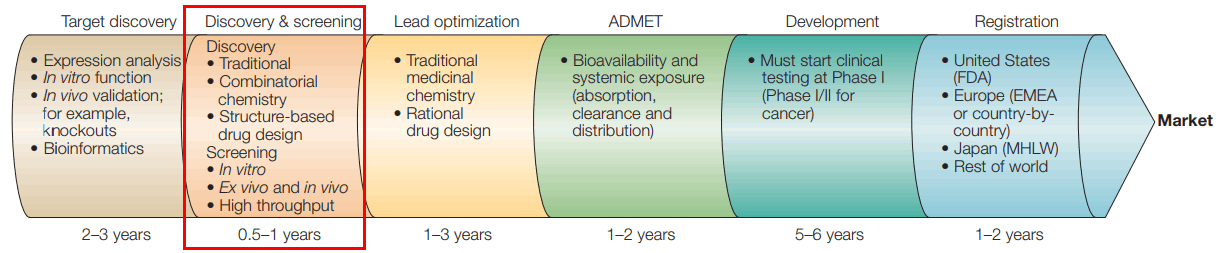
\includegraphics[width = \textwidth]{../figures/pipeline_1.png}\\
 {\centering \scriptsize General process and time line for drug development \footnotemark[1]}
\begin{itemize}
    %==  as shown in the figure below
    \item The full drug discovery and development takes 10-17 years with a less than 10\% overall probability of success
    %==  success as defined by, eventually approved by FDA and make it to the market
    %==  therefore, there is always motivation to "start right", or "start better" with a compound that is more likely to pass the subsequently ADMET tests
    %==  in which leads to:
    \item Computer aided drug design (CADD) \textit{Discovery \& screening}: virtual screening
    %==  following the step of target identification
    %==  in which step, the target of the disease is identified
    %==  target is officially defined as a bio-chemical entity, that when combined with drugs, unergoes a specific interaction that has connection with clinical effects.
    %==  (this is an older illustration graph),
    %==  with the development of computer science, it's taking a role in drug discovery in the screening step which is termed as 'in silico' virtual screening
    %==  Virtual screening (VS) is a computational technique used in drug discovery to search libraries of small molecules in order to identify those structures which are most likely to bind to a drug target
    %== it helps decide which compunds to sythesise, test for ADMET properties next
    \item Key component of virtual screening: molecular docking
    %== here introduce my motivation for this proposal: better molecular docking results that will eventually to applied to virtual screening of a real-scenario target
    \end{itemize}
 \footnotetext[1]{Ashburn, Ted T., and Karl B. Thor. "Drug repositioning: identifying and developing new uses for existing drugs." Nature reviews Drug discovery 3.8 (2004): 673.}
\end{frame}


%==%%%%%%%%%%%%%%%%%%%%%%%%%%%%%%%%%%%%%%%%%%%%%%%%%%%%%
\subsection{Innovation}
\begin{frame}{Innovation: machine learning assisted virtual screening}
    \begin{columns}
    \begin{column}{0.4\textwidth}
  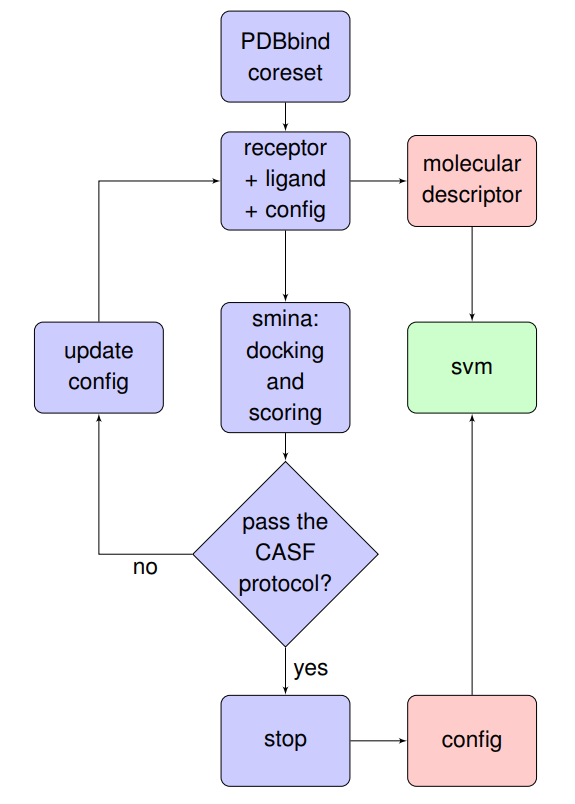
\includegraphics[height = 0.8\textheight]{../figures/innovation.png}\\
 {\scriptsize Work flow of the machine learning architecture}
    \end{column}   
    \begin{column}{0.55\textwidth}
    \begin{block}{Deficiency in virtual screening process}
    Lack of tuning between the \textbf{docking software} and \textbf{batch screening process}
    %== this proposal targets at improveing the accuracy of virtual screening results,
    %== as my research into virtual screening shows that,
    %== there are researchers spending a lot effort building more "accurate" scoring functions for molecular docking
    %== there are researchers writing protocol for evauluating the functionality of newly developed scoring functions
    %== and people have, published numerous amounts of literature debating on which docking software performs better on which benchmark datasets
    %== there are researchers developing standard operating procedure for performing virtual screening
    %== but it lacks customize between docking and virtual screening
    \end{block}
    \pause
    \begin{block}{Aim 1: machine learning tuned docking parameters}
    %== this proposal adds an additional step between within the virtual screening process to costomized the screening for better resutls.
    The characteristic of the receptor and ligand will be learned for virtual screening
    \end{block}
    \begin{block}{Aim 2: active learning selection of ligands}
    %== this proposal adds an additional step between within the virtual screening process to costomized the screening for better resutls.
    Instead of going through ligand library in a random order, machine learning algorithm is used to learn which un-tested ligand will be the mostly likely binder
    \end{block}
    \end{column} 
    \end{columns}

\end{frame}


%==%%%%%%%%%%%%%%%%%%%%%%%%%%%%%%%%%%%%%%%%%%%%%%%%%%%%%%%%%%%%%%
\section{Background}
\subsection{Virtual screening}
\begin{frame}{Pipeline for virtual screening}
   \begin{columns}
    \begin{column}{0.45\textwidth}
    \begin{block}{Steps for the practice of receptor-based virtual screening}
    %== the general framework for in silico virtual screening is illustrated in this figure
    %== the actual screening part, which is, step #3
    %== is categorized into ligand based or receptor-based.
    %== when looking at a specific practical screening scenario
    %== researchers first evauluate: do we have a high resolution structure of the receptor?
    %== if so, use the receptor-based virtual screening
    %== if not, follow through the ligand based virtual screening, which involves different kind of modeling of the probelm
    %== in my proposal, i assume that i have the structure of the receptor
    %== therefore virtual screening will rely on molecular docking
    \begin{enumerate}
      \item Target identification: find the protein that serves a role in the disease in interest
      \item File preparation (3D structure of the protein and the ligands in the library to be screened)
      \item Docking and ranking by docking software
      \item ADMET (absorption, distribution, metabolism, excretion, and toxicity) evaluation
    \end{enumerate}
    %== to describe the general pipeline of the virtual screening process
    %== first the protein needs to be identified
    %== second, the 3d structure should be downloaded and preprocessed
    %== third define the active site , along with 3d structures and perform molecular docking
    %== ligands with high binding affinitys ouputed by the software
    \end{block}
    \end{column}   
    \begin{column}{0.4\textwidth}
        \hfill
        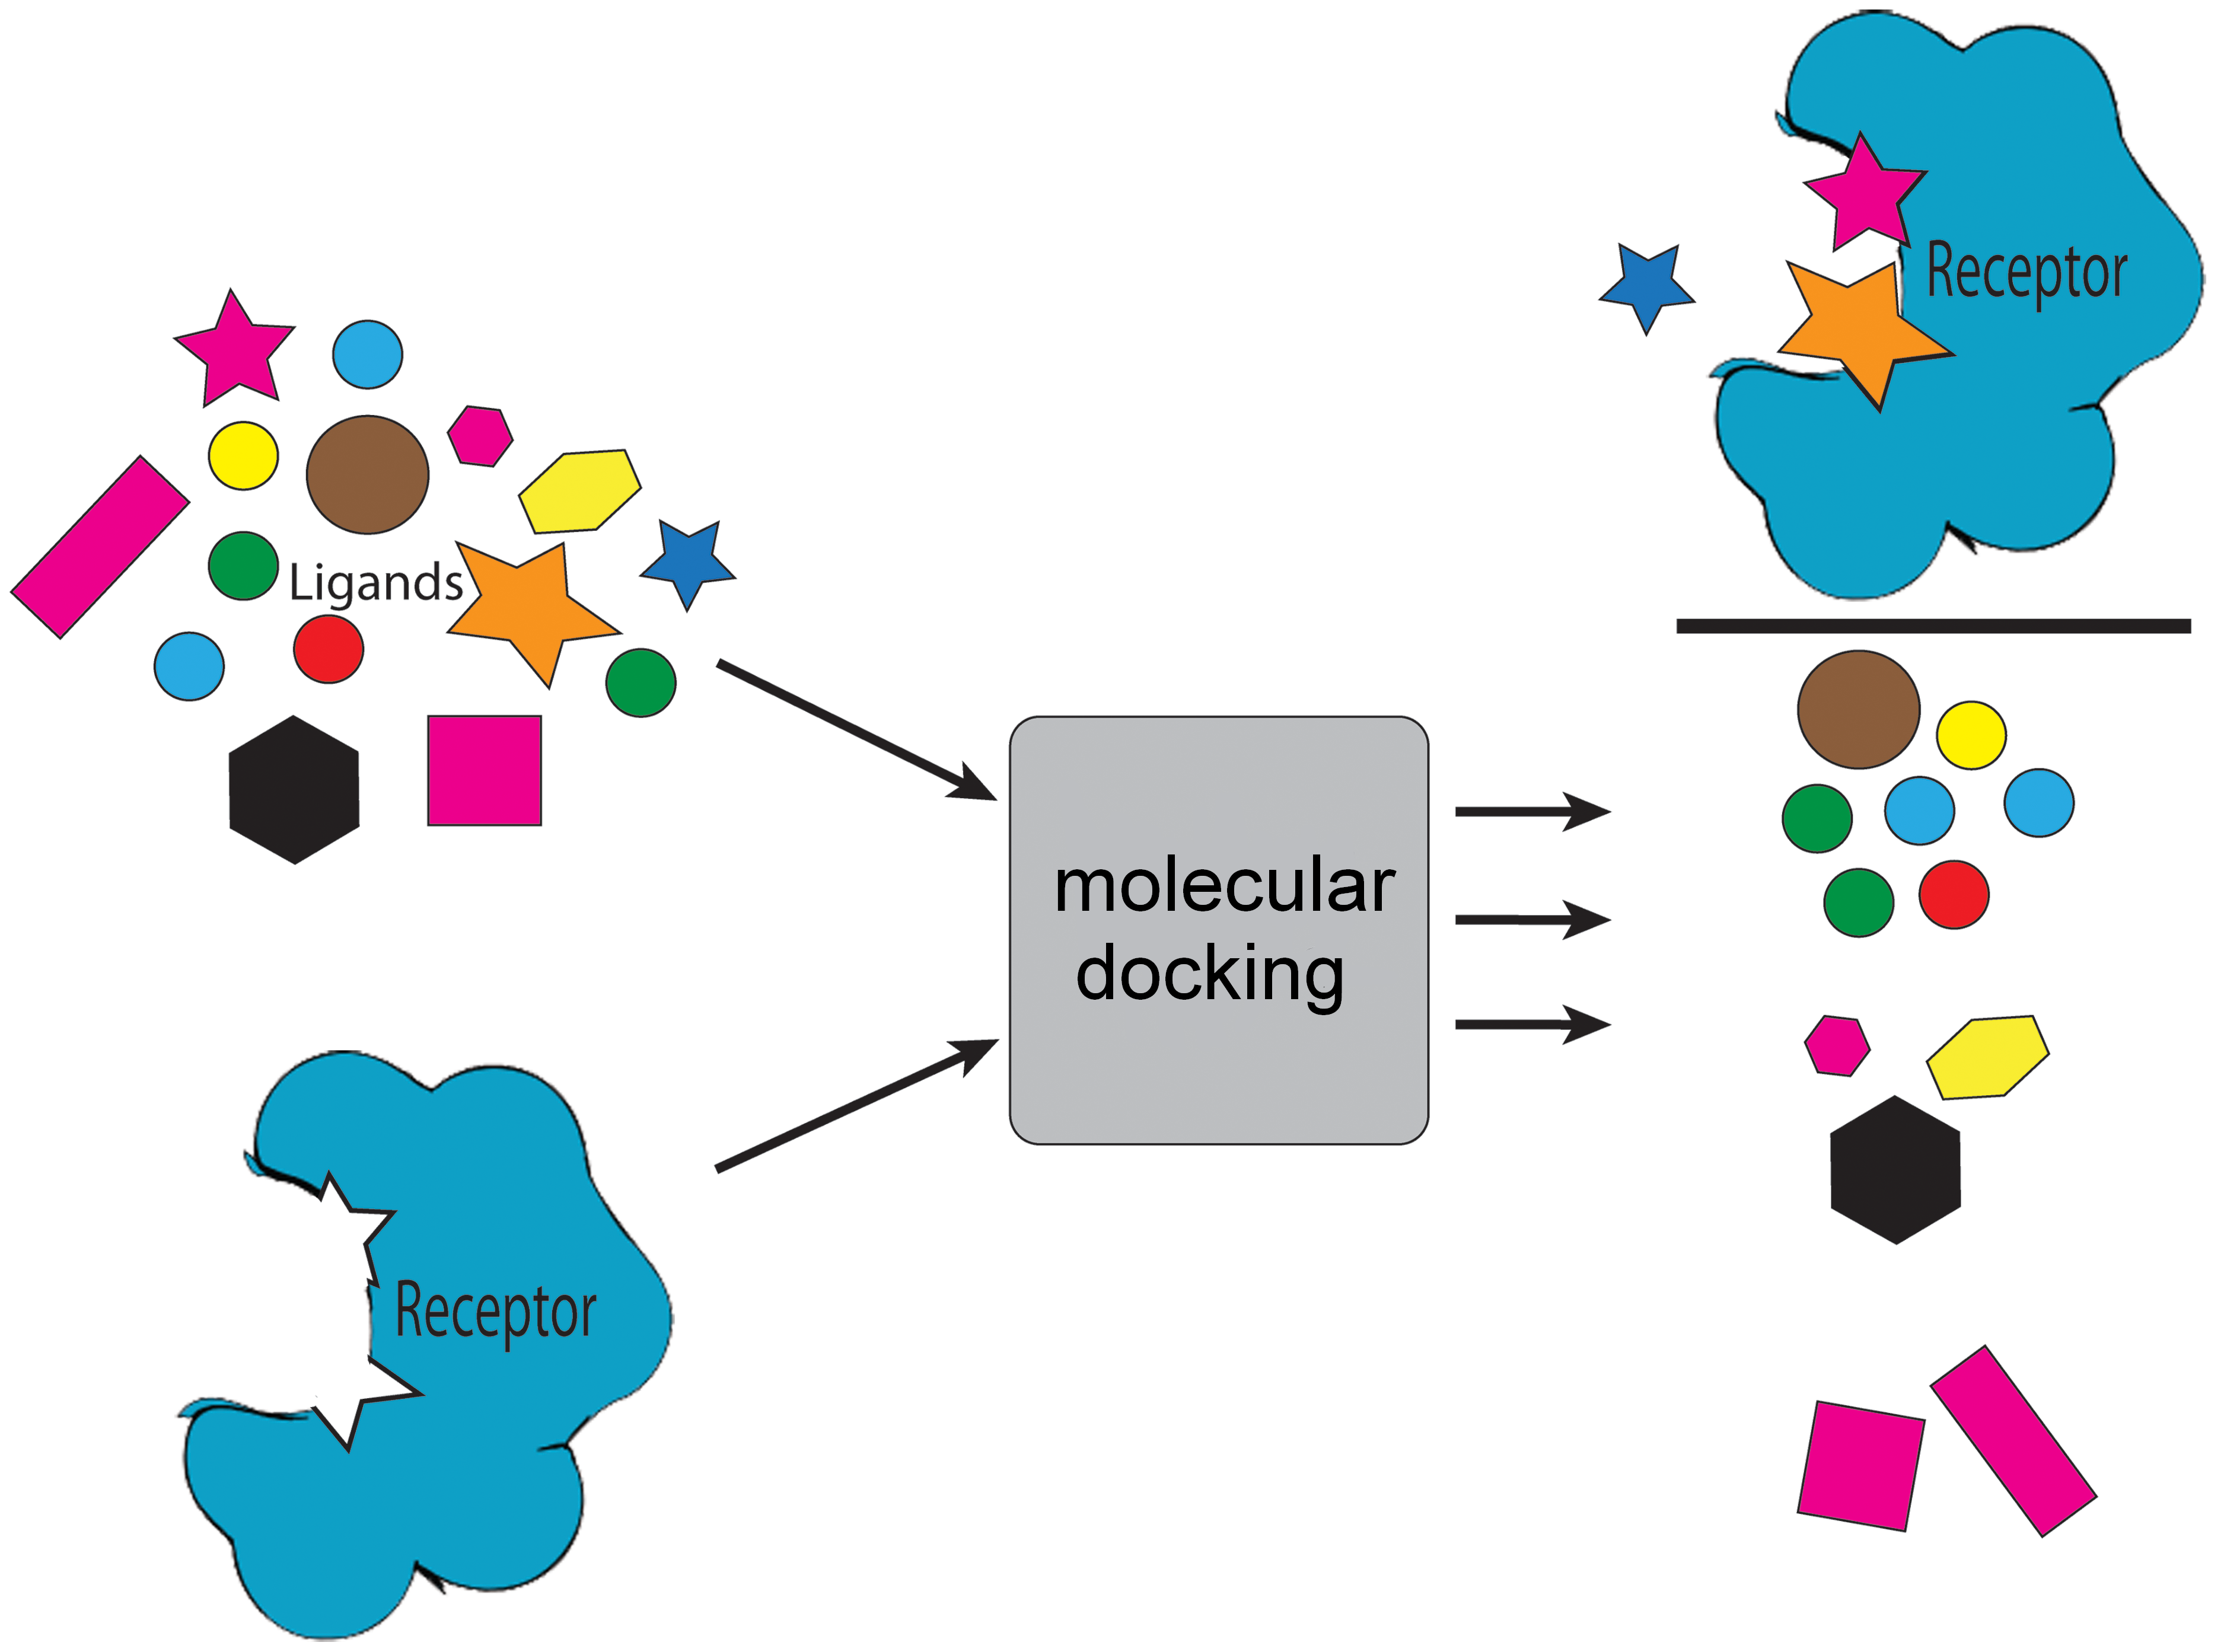
\includegraphics[width=\textwidth]{../figures/vs1.png}\\
      {\hfill \scriptsize Illustration of  \textit{in silico} small molecule screening}
    \end{column}
    \end{columns}
\end{frame}

\subsection{Molecular docking}
\begin{frame}{Three questions for molecular docking}
   \begin{columns}[T]

   \begin{column}{.4\textwidth}
   %== the figure on the left describes the basic concept of molecular docking
   %== which is, given the 3d structure of the receptor and the ligand
   %== evaluate how the two bind into one entity
        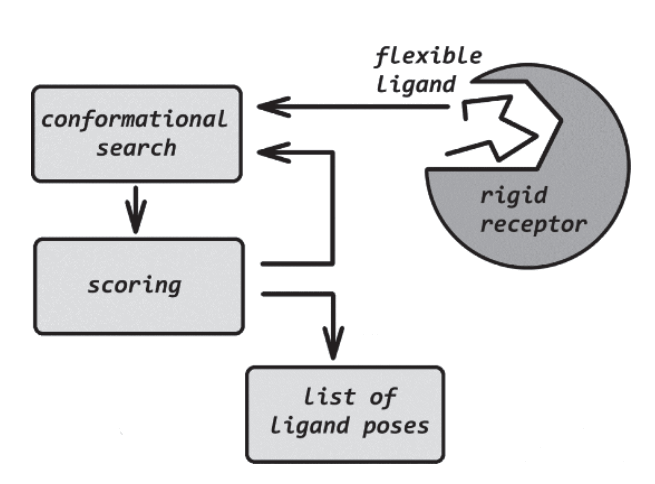
\includegraphics[width=\textwidth]{../figures/md_process.png}\\
      {\scriptsize Principal scheme of a molecular docking procedure \footnotemark[1]}
\end{column}

\begin{column}{.55\textwidth}
    \begin{block}{Sampling question}
    %==  When referring to molecular docking, generally it is defined as: Computational approaches that 'dock' small molecules into the structures of macromolecular targets and 'score' their potential complementarity to binding sites are widely used in hit identification and lead optimization
    %==  when practically performing a molecular docking event, these are the aspects that we want to the dockign software to give us answers to
    %==  first is,  
What pose will this ligand dock to the receptor?
%== this is sometimes termed as, the orientation, conformation, sampling 
%== the difficulty of the sampling question scales with how much flexibility the ligand and the receptor has
%== this step is performed by the docking software normally using a genetic algorithm, or monte carlo algorithm
    \end{block}   
    \pause
    \begin{block}{Scoring question}
%== task number 2, accurately predit the binding affinity of a small molecular from receptor-ligand interactions.
what is the binding affinity of an  selected receptor-ligand pose?\\
%== this is normally referred to as the scoring question
%== the scoring functions are used both to guide sampling, and to rank the sampled poses
%== scoring function are categorized into force field based, knowledge based, and empirical ones
%== force-field ones seek to quantify the actual molecular forces that exist between the ligand and the receptor, accounting for van der waals interactions, electrostatic interactions and hydrogen bonding interactions
%== knowledge based seek to derive simplified potentials directly from databases of structural data, which often end up in a pair wise addition of atoms in the same neighborhood
%== empirical incorporate dlements of both mentioned above,, they consit of phusically meaningful terms that are parameterized, they are somewhat similar to force field terms but also contains more complicated- not- modellable terms. They are trained on co-crystalized structure with known binding affinities, therefore it's highly dependant on the training data.
%== with the progression of computer science, recent years has seen machine learning based scoring functions, they are sometimes catergorized into the empirical categoried, there are also literature put them into a 4th category: descriptor based scoring functions. 
%== Both catory makes sense somehow, 1st, "machine learn" meaning training, the there is a physical model of converting the interaction between the ligand and the receptor into descriptors, in which case 'descriptor based is also appropriate, because machine learing relys on the numerated descrptors, and depending the descriptor intepretation, the major trends on this category have employed 
%== k-nearst neighbor, naive bayes, random foreset -> decision tree, support vector machine, nerural network, convolution network
%== there are different methodalogies, i will elaborate on svm, which will be the method i use for learning, please note that this is a different scenario than to implement the machine learning in the actual scoring function.
%== as the current development:  most docking programms 
%== reasonably good at finding the correct pose for a given protein-ligand complex
%== less good at ranking different ligands aginst the same protein (which arises problem in virtual screening)
    \end{block}
    \pause
     \begin{block}{Decision}
is this putative ligand a `binder' or `non-binder'?
%== in this case, when you set if the binding affinity exseeds certain amount, it can be clssified as a binder or non binder
    \end{block}
\end{column}
    \end{columns}
    \footnotetext[1]{Lo, Yu-Chen, et al. "Quantitative Methods in System-Based Drug Discovery." Complex Systems, Sustainability and Innovation. InTech, 2016.}
\end{frame}


%==%%%%%%%%%%%%%%%%%%%%%%%%%%%%%%%%%%%%%%%%%%%%%%%%%%%%%%%%%%%%%%
\section{Aim 1}
\subsection{Description}
\begin{frame}{Aim 1: Optimized docking parameters in virtual screening}
   \begin{columns}
    \begin{column}{0.45\textwidth}
\begin{block}{Aim 1}
Additional step prior to screening: parameters optimization
\end{block}
\begin{block}{Methodology}
Generate molecular descriptor and corresponding docking parameters and build a docking parameter predictor with SVM
\end{block}
%== here is my first proposal
%== instead of the simple virtual screening pipleline as described above, and as practiced routinely,
%== the docking parameters will be trained prior
%== instead of just feeding the ligands into the docking software
%== each input ligand will have different docking parameters
    \end{column}   

    \begin{column}{0.4\textwidth}
        \hfill
        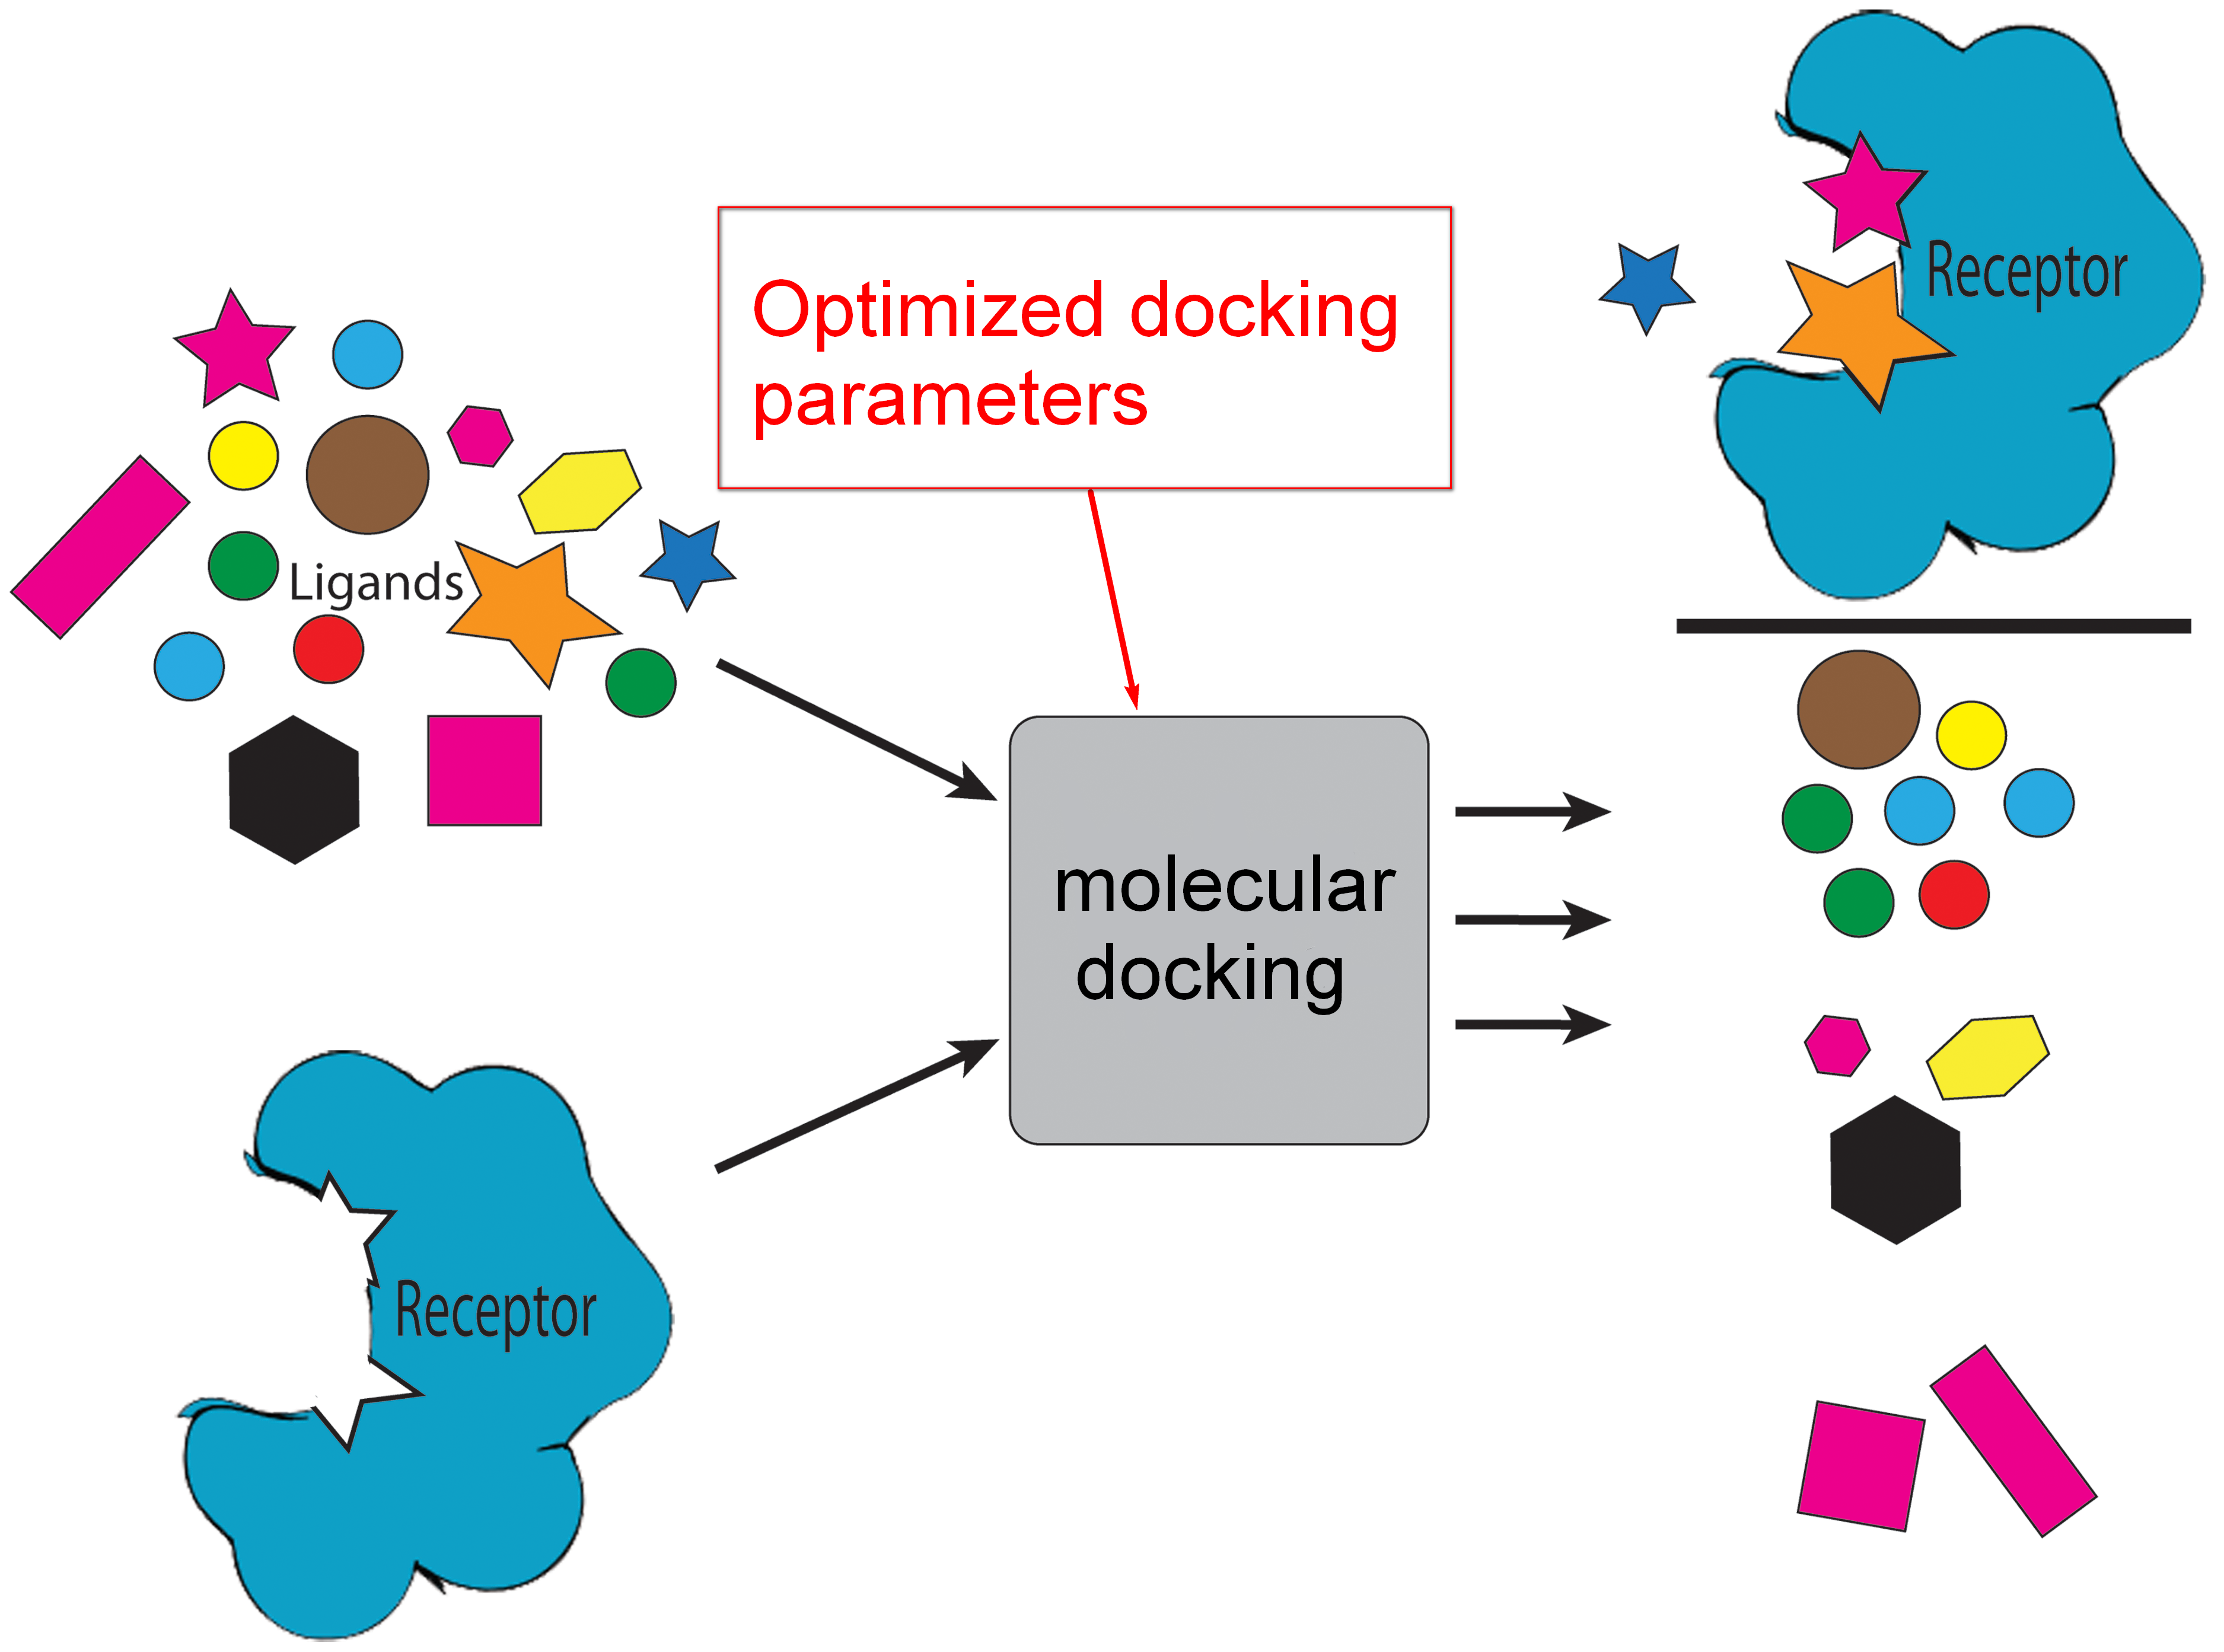
\includegraphics[width=\textwidth]{../figures/vs2.png}\\
      {\hfill \scriptsize Additional docking parameters in the framework}
    \end{column}
    \end{columns}
\end{frame}

\subsection{Implementation}


\begin{frame}[fragile]
\frametitle{Implementation of Aim 1: smina, user-defined empirical scoring function}
   \begin{columns}
       \begin{column}{0.4\textwidth}
        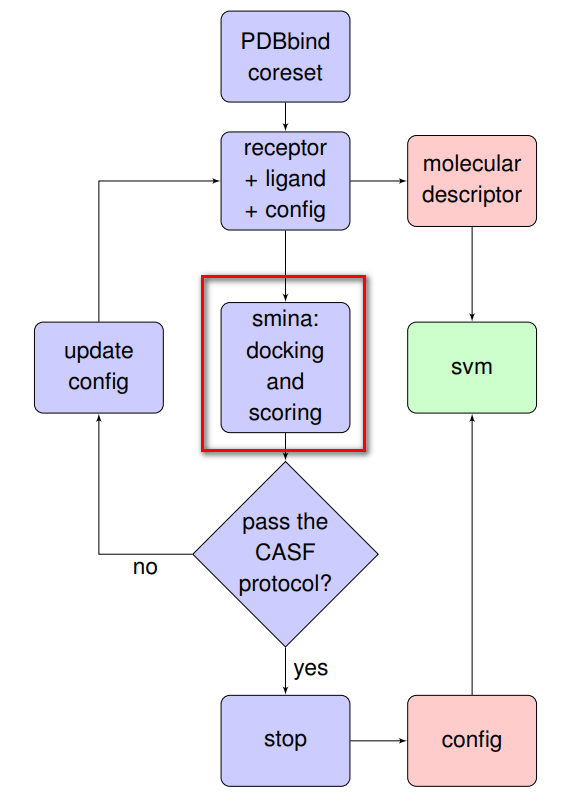
\includegraphics[height=0.8\textheight]{../figures/method_smina.png}\\
      {\scriptsize Work flow of updating configuration}
    \end{column}
%== for performing the docking, here i use smina, not necessaily smina
%== smina is a fork of the famous autodock vina
%== usage of smina rather than vina, is because it goes into vina and offered more tweaking parameters for user to define
%== here offers a abbreviated list of the user defined parameters
%== the author of smina phrased this as the 'user-defined' scoring function, because when comparing to vina, vina only offers running parameters of : search box location,  number of cpu to use, random seed, exhaustiveness of the search, number of modes, and the energy range
%== whereas in smina, below is just a subset of parameters that can be specified.
%== 1.0 at beginning of each line is the weights to be put onto the parameter specified.
%== the full weights list will be the configuration that's updated is the docking software does not pass the CASF evaluating protocol
%== I plan to random updating scheme initially,
%== but further investigation can be done to construct a hierrachy of the list
    \begin{column}{0.55\textwidth}
\begin{block}{Smina: user defined scoring function}
\begin{lstlisting}[language={},caption = smina user defined parameters example, frame=single]
1.0  num_tors_add
1.0  num_tors_sqr
1.0  num_tors_sqrt
1.0  ligand_length
\end{lstlisting}
\end{block}
    \end{column}   
    \end{columns}
\end{frame}

\begin{frame}
\frametitle{Implementation of Aim 1: CASF benchmark dataset}
   \begin{columns}
       \begin{column}{0.4\textwidth}
        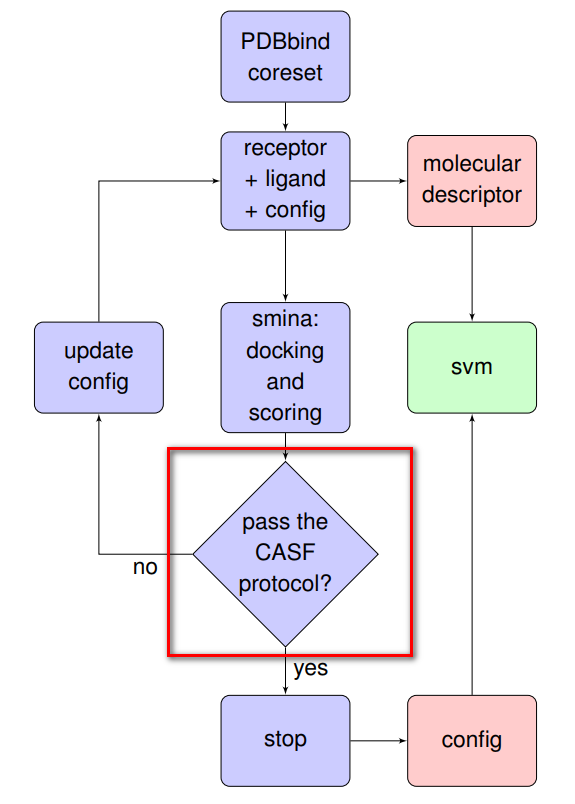
\includegraphics[height=0.8\textheight]{../figures/method_casf.png}\\
      {\scriptsize Work flow of updating configuration}
    \end{column}
    %== on this left is my architechture for aim 1
    %== to begin with, i want optimized docking parameters
    %== to what standard that i optimize to parameters to?
    %== CASF! same ppl maintaining the PDBbind dataset.
    %== btw, pdbbind is a database, that include the protein-ligand and bio experimental datasets
    %== they newly published a protocol on how to use a refinemnet core set of complexes to evaulate the functionality a newly developed scoring functions
    %== as mentioned above, docking = sampling + scoring
    %== these two functionalities are tested as the powers as listed 
    %== they are conveniently written into bash scripts and outputs as numbers for evaulations.
    %== therefor, i will initially use the default parameters to dock
    %== raise output by (e.g. 10%) and the pass threshold
    \begin{column}{0.55\textwidth}
\begin{block}{Comparative Assessment of Scoring Functions}
    CASF is a protocol designed to evaluate the functionality of newly developed docking softwares.\\
    Core set: tested dataset consists of 195 protein-ligand complexes in 65 protein clusters, each cluster containing a representative of 3 complexes that span 10 orders of magnitude in binding affinity.\\
    \begin{itemize}
      \item Scoring power: production of `accurate' binding affinity
      \item Ranking power: rank ligands correctly
      \item Docking power: identify native binding pose among decoy poses
      \item Screening power: high enrichment factor
    \end{itemize}
    \end{block}
    \end{column}
    \end{columns}
\end{frame}






\begin{frame}{Implementation of Aim 1: molecular descriptors}
%== this step uses RDKit to transfer the properties of ligand into molecular descriptors.
%== RDKit is waht i identified as a mature packages that can be easily incooporate into the pipeline, but alternative molecular descriptor can be used in this step as well.
   \begin{columns}
       \begin{column}{0.4\textwidth}
        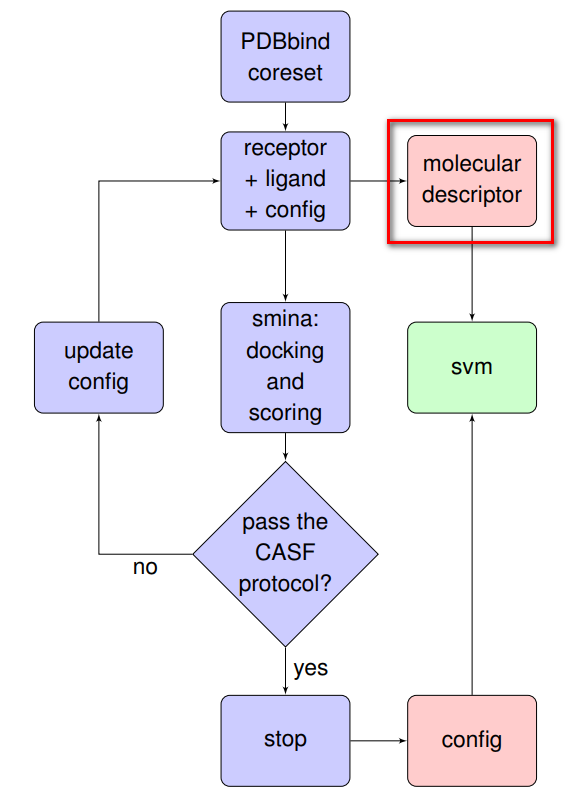
\includegraphics[height=0.8\textheight]{../figures/method_rdkit.png}\\
      {\scriptsize Work flow of updating configuration}
    \end{column}
    \begin{column}{0.55\textwidth}
\begin{block}{Dragon for generation of molecular descriptors}
%== to describe what is molecular descriptor, it converts the molecular structrue into computer recognizable language
%== below offers an example of how molecular descriptor works that i find to be illustratable with simplified equations
For both the protein P and the ligand L:
\begin{equation*}
\begin{aligned}
\{ P(j)\}_{j=1}^9 &= \{C,N,O,F,P,S,Cl,Br,I\} \\
\{L(i)\}_{i=1}^9 &= \{C,N,O,F,P,S,Cl,Br,I\}
\end{aligned}
\end{equation*}
The occurrence count for a particular j-i atom type pair is defined as:
\begin{equation*}
\varkappa _{Z(P(j)),Z(P(i))} \equiv \sum_{k=1}^{K_j} \sum_{l=1}^{L_i} \Theta (d_{cutoff}-d_{kl})
\end{equation*}
%== this is a pair wise, distance-dependant addtion method, which is common for machine learning based scoring functions(but that's not really relevant in this scenario)
%== cuttoff = 12, 12 angstrom within the neighborhood
%== j, i specifis atom types
%== K,L total number of
%== Z returns the number count
\end{block}
    \end{column}
    \end{columns}
\end{frame}

\begin{frame}{Implementation of Aim 1: Supporting Vector Machine}
   \begin{columns}
          \begin{column}{0.4\textwidth}
        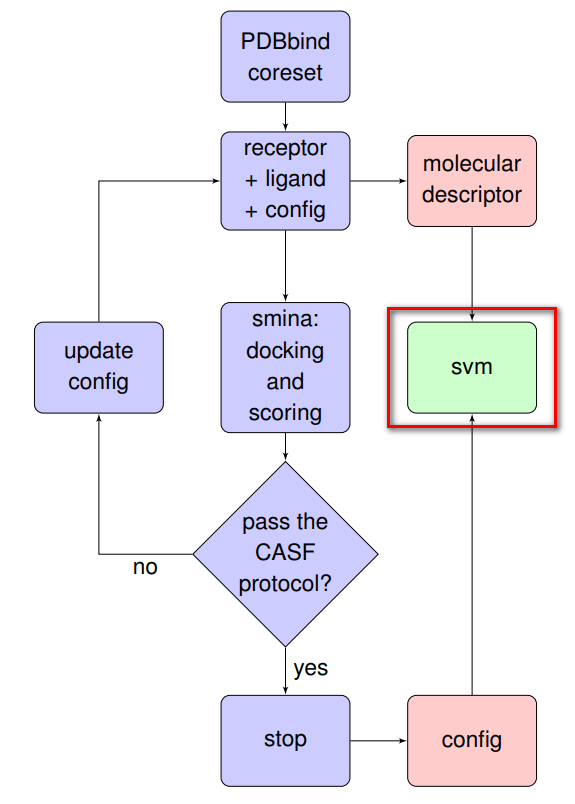
\includegraphics[height=0.8\textheight]{../figures/method_svm.png}\\
      {\scriptsize Work flow of updating configuration}
    \end{column}
    \begin{column}{0.55\textwidth}
              \centering
    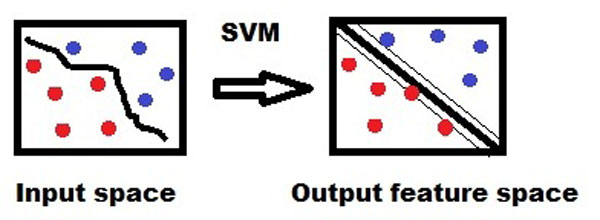
\includegraphics[width=0.6\textwidth]{../figures/concept_svm.png}\\
      {\scriptsize Concept of SVM}
\begin{block}{Concept of Supporting Vector Machine (SVM)}
Kernel function project data to higher dimension (feature dimension)\\
Mathematically, only one hyperplane can separate the data with closest data (supporting vectors)\\
Regression model: solve hyperplane, such that data center around it, return function of the hyperplane
\end{block}
\begin{block}{SVM predictor}
%== for this step, i plan to use svm that's packages in matlab, sklearn, or tensorflow, since i will have 195 training data sets
%== to explain svm conceptually, consider the plot on the top right 
%== data that's linearly un-separatable becomes linearly separatable in the fearture space
%== briefly, svm project input data into a higher dimension using a kernel function
%== the linear separation line is termed as hyper plane.
%== relys on the unlinearity of the kernel function, actually depend on the charasteristic of the data, which could would be investigated as in which one to use, but i plan to use the Raial basis fucntion kernel
Given putative ligand, out-put optimal docking parameters
\end{block}
    \end{column}
    \end{columns} 
\end{frame}

%==%%%%%%%%%%%%%%%%%%%%%%%%%%%%%%%%%%%%%%%%%%%%%%%%%%%%%%%%%%%%%%
\section{Aim 2}
\subsection{Description}
\begin{frame}{Aim 2: Active learning in screening}
\centering  
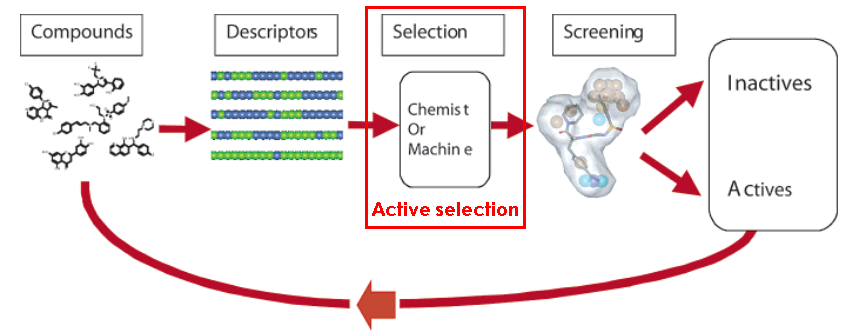
\includegraphics[width = 0.75\textwidth]{../figures/active.png}\\
 {\scriptsize The drug screening cycle \footnotemark[1]}

\begin{block}{Aim 2: active selection with SVM}
%== two terms, active slection vs bio-active
%== svm, some concept, with different application
%== firt, svm is used in this situation as a classification of binder or non binder, ranther than a regression problem as descibed for the architechture in aim 1
Instead of randomly screening through the ligand library, tested ligands will be labeled as `binders' or `non-binders' and project into higher space, in which a hyperplane will be drawn, the next ligand to be docked will be the one that's most positive
\end{block}
\footnotetext[1]{Warmuth, Manfred K., et al. "Active learning with support vector machines in the drug discovery process." Journal of chemical information and computer sciences 43.2 (2003): 667-673.}
\end{frame}

\subsection{Implementation}
\begin{frame}{Implementation of Aim 2: SVM}
  \begin{columns}[T]
  \begin{column}{0.45\textwidth}
  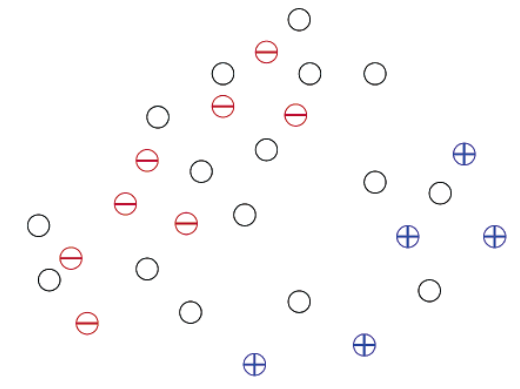
\includegraphics[height = 0.4\textheight]{../figures/svm1.png}\\
 {\scriptsize Three types of data points in two-dimensional descriptor space \footnotemark[1]}
 \begin{block}{Putative ligand type}
 Blue: binders\\
 Red: non-binders\\
 Black: un-tested data
 \end{block}
\end{column}
\begin{column}{0.45\textwidth}
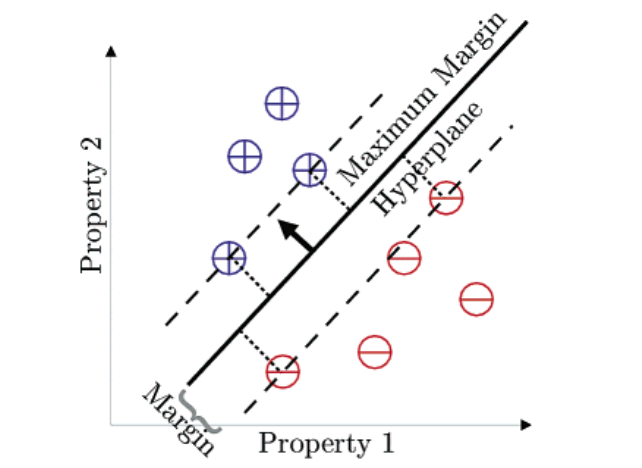
\includegraphics[height = 0.4\textheight]{../figures/svm2.png}\\
 {\scriptsize Data mapped with maximum margin hyperplane \footnotemark[1]}
  \begin{block}{Active selection}
 The most positive ligand will be docked next
 \end{block}
\end{column}
\end{columns}
\footnotetext[1]{Warmuth, Manfred K., et al. "Active learning with support vector machines in the drug discovery process." Journal of chemical information and computer sciences 43.2 (2003): 667-673.}
\end{frame}

\subsection{Evaluation}
\begin{frame}{Two fold evaluation of this virtual screening architecture}
\begin{block}{Evaluation for the docking parameter predictor: three fold cross validation}
Dividing the 195 complexes into 3 subsets, with mixed binding affinities\\
Cross validation method: leave-one-out cross-validation
\end{block}
\begin{block}{Directory of Useful Decoys, Enhanced}
102 targets, 22886 clustered ligands\\
Performs simulated virtual screening using the DUD$\cdot$E benchmark datasets\\
Evaluate before\&after ROC, AUC plots 
\end{block}
\end{frame}

%==%%%%%%%%%%%%%%%%%%%%%%%%%%%%%%%%%%%%%%%%%%%%%%%%%%%%%%%%%%%%%

\section{Aim 3}
\subsection{Description}
\begin{frame}{Aim 3: application of this virtual screening architecture with receptor related to Alzheimer's Disease (AD)}

\begin{block}{Aim: to applicate the system}
Potential drug: acetylcholineterase inhibitors (AChEI)\\
Identified targets: BACE1, the M1 subtype of mAChR, APP, CDK5, and GSK-3$\beta$
\end{block}

\begin{block}{Evaluation}
Comparison to recent advances in AChEI using other machine learning virtual screening methods
\end{block}


\end{frame}








%==%%%%%%%%%%%%%%%%%%%%%%%%%%%%%%%%%%%%%%%%%%%%%%%%%%%%%%%%%%%%%
%==%%%%%%%%%%%%%%%%%%%%%%%%%%%%%%%%%%%%%%%%%%%%%%%%%%%%%%%%%%%%%
\section{Concluding remarks}

%==%%%%%%%%%%%%%%%%%%%%%%%%%%%%%%%%%%%%%%%%%%%%%%%%%%%%%%%%%%%%%
\subsection{Conclusion}
\begin{frame}{Concluding remarks}
\begin{itemize}
    \item Simple architecture with additional tuning using machine learning algorithm
    \item No theoretical foundation into the scoring function to evaluate whether the configuration update will converge
\end{itemize}
\end{frame}

%==%%%%%%%%%%%%%%%%%%%%%%%%%%%%%%%%%%%%%%%%%%%%%%%%%%%%%%%%%%%%%%
\subsection{Questions?}
\begin{frame}[label=questions]
Questions?

  \hyperlink{additional}{\beamerreturnbutton{Additional Information}}
\end{frame}


% Computational approaches that 'dock' small molecules into the structures of macromolecular targets and 'score' their potential complementarity to binding sites are widely used in hit identification and lead optimization
% \hyperlink{questions}{\beamerreturnbutton{return}}

\appendix

\begin{frame}[label=additional]{Additional information}
  \tableofcontents
\end{frame}



%%%%%%%%%%%%%%%%%%%%%%%%%%%%%%%%%%%%%%%%%%%%%%%%%%%%%%%%%%%%%%%%%%%%%%%%%%%%%%%%%%%%%%%%%%%%%%%%%%%%%%%%%
\section{Structure based drug design}
\begin{appendixframe}{System based  drug  discovery methods}
System based  drug  discovery  can  be classified  as  ligand-based  and  structure-based
\begin{itemize}
\item Ligand-based: only  ligand  information  is  used  to  derive  its  multitude  of chemical and biological properties
\item  Structure-based: use the structure of the receptor to identify shape-complementary ligands with optimal interactions
\end{itemize}
The structure-based drug design process is as follows:
\begin{itemize}
\item An enzyme that is important in a particular pathological condition is chosen
\item The three-dimensional structure of the active site of the enzyme is determined, often by X-ray crystallography
\item A chemical is prepared to fit the active site of the enzyme, which can alter the properties of the enzyme
\end{itemize}
\textbf{Key feature for structure based: accurate structure file of the receptor}
\end{appendixframe}





%%%%%%%%%%%%%%%%%%%%%%%%%%%%%%%%%%%%%%%%%%%%%%%%%%%%%%%%%%%%%%%%%%%%%%%%%%%%%%%%%%%%%%%%%%%%%%%%%%%%%%%%%%%%%%%%%%%%%%%%
\section{Scoring function categories}
\begin{appendixframe}{Scoring function categories}
\centering
\textbf{Force field based scoring functions}
\begin{columns}[T]
\begin{column}{0.4\textwidth}
Based on physical atomic interactions such as:
\begin{itemize}
    \item van der Waals interaction
    \item electrostatic interactions
    \item bond stretching/bending/torsional forces
\end{itemize}
Derived from experimental data and quantum mechanical calculations and made with assumptions.
\end{column}

\begin{column}{0.4\textwidth}
\begin{equation*}
E = \sum_{\substack{i}}\sum_{\substack{j}} (\frac{A_{ij}}{r^{12}_{ij}} - \frac{B_{ij}}{r^{6}_{ij}} + \frac{q_i q_j}{\epsilon (r_{ij})r_{ij}}) 
\end{equation*}
\begin{itemize}
    \item i,j denotes atom number
    \item A, B van der Waals parameters
    \item q denotes atom charges
\end{itemize}
Limitation:
\begin{itemize}
    \item Computationally expensive to account for solvent effect 
    \item Empirical weighting 
\end{itemize}
\end{column}
\end{columns}
\end{appendixframe}



%%%%%%%%%%%%%%%%% empirical scoreing

% estimate the binding affinity of a complex
% on the basis of a set of weighted energy terms




%%%%%%%%%%%%%%%%% knowledge based
% potentials in eqn (3)
% are extracted from the structures rather than from attempting
% to reproduce the known affinities by fitting,

% Most of the current knowledge-based scoring functions
% approximate the reference state with an atom-randomized
% state by ignoring the effects of excluded volume, interatomic connectivity, etc.88 Gohlke et al. developed a knowledge-based
% state by ignoring the effects of excluded volume, interatomic connectivity, etc.88 Gohlke et al. developed a knowledge-based
% scoring function (DrugScore) based on 17 atom types and 1376 protein–ligand complex structures.41 The scoring func-scoring function (DrugScore) based on 17 atom types and 1376 protein–ligand complex structures.41 The scoring func-tion consists of a distance-dependent pair-potential term and a
% surface-dependent singlet-potential term.

% The problem is more prominent for binding mode
% predictions and virtual screening, as the pairwise potentials,
% which are derived from nicely-bound structures, are not
% sufficiently sensitive to different ligand positions and may give
% good scores even to bad/wrong modes.


% circumvent the accurate calculation of the reference state.36,37,99–101 The basic
% idea of the iterative method is to adjust the pair potentials uij(r) by iteration until the interaction potentials reproduce the
% idea of the iterative method is to adjust the pair potentials uij(r) by iteration until the interaction potentials reproduce the
% experimentally determined pair distribution function in the
% training set, yielding a set of potentials that can discriminate the native structures from decoys.102–105 During the iteration
% training set, yielding a set of potentials that can discriminate the native structures from decoys.

\begin{appendixframe}{Scoring function categories}

\begin{columns}[T]
\begin{column}{0.45\textwidth}
\textbf{Knowledge-based (statistical-potential)}\\
Principal: inverse Boltzmann relation
\begin{equation*}
w(r) = - k_B t \ln [g(r)], ~ g(r) = \rho (r)/\rho^\ast (r)  
\end{equation*}

\begin{itemize}
    \item $k_B$ Boltzmann constant
    \item $T$: absolution temperature
    \item $\rho(r)$: atom pair number density at distance $r$
    \item $\rho^\ast(r)$: density in reference state % where the interatomic interactions are 0
    \item $g(r)$ pair distribution function
\end{itemize}
Challenge: description of reference state
\end{column}
\hspace{1em}
\begin{column}{0.45\textwidth}
\textbf{Empirical scoring functions}
\begin{equation*}
\Delta G = \sum_{\substack{i}} W_i \cdot \Delta G_i \footnotemark[1]
\end{equation*}

\begin{itemize}
    \item $\Delta G_i$ represents different energy terms
    \item Corresponding coefficients $W_i$ determined by fitting training data sets
\end{itemize}

Compare to force filed scoring functions: 
\begin{itemize}
    \item Simple and fast
    \item Training set: 200
\end{itemize}
\end{column}
\end{columns}
\footnotetext[1]{Huang, Sheng-You, Sam Z. Grinter, and Xiaoqin Zou. "Scoring functions and their evaluation methods for protein–ligand docking: recent advances and future directions." Physical Chemistry Chemical Physics 12.40 (2010): 12899-12908.}
\end{appendixframe}


\section{SVM}
\begin{frame}{Why SVM}
\centering
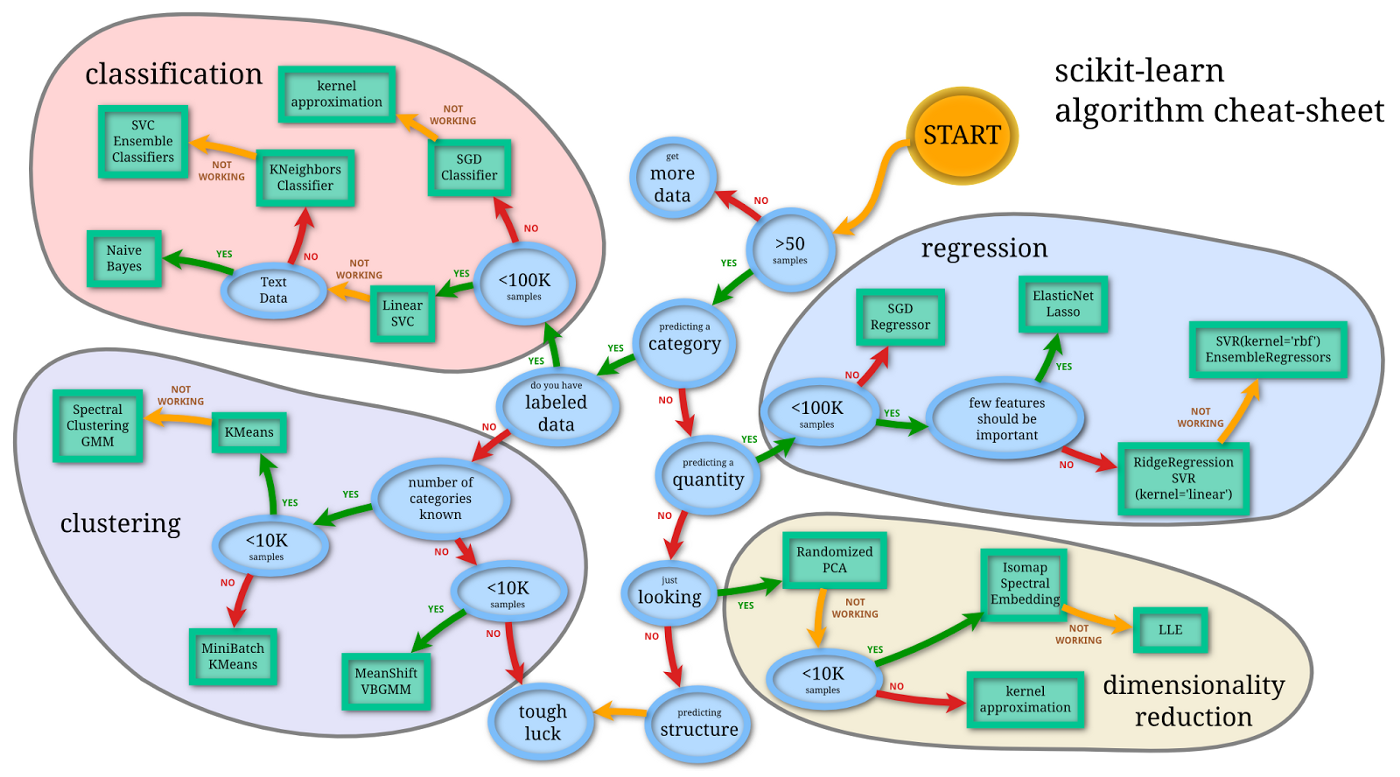
\includegraphics[height=0.8\textheight]{../figures/ml_cheatsheet.png}
\end{frame}

\begin{frame}{SVM for regression}
\begin{block}{Classification vs regression}
Classification: hyperplane separates different classes\\
Regression: hyperplane cluster the data sets
\end{block}
\end{frame}

\begin{frame}[fragile]
\frametitle{SVM usage}
\begin{block}{Model fitting example}
\begin{lstlisting}[language={python},frame=single]
from sklearn import svm
X = [[0, 0], [1, 1]]
y = [0, 1]
clf = svm.SVC(gamma='scale')
clf.fit(X, y)  
SVC(C=1.0, cache_size=200, class_weight=None, coef0=0.0,
    decision_function_shape='ovr', degree=3, gamma='scale', kernel='rbf',
    max_iter=-1, probability=False, random_state=None, shrinking=True,
    tol=0.001, verbose=False)
\end{lstlisting}
\end{block}
\begin{block}{Prediction of new value}
\begin{lstlisting}[language={python},frame=single]
clf.predict([[2., 2.]])
array([1])
\end{lstlisting}
\end{block}
\end{frame}


\end{document}









